\documentclass[conference]{IEEEtran}
\IEEEoverridecommandlockouts

\usepackage{cite}
\usepackage{amsmath,amssymb,amsfonts}
\usepackage{graphicx}
\usepackage{textcomp}
\usepackage{xcolor}
\usepackage{booktabs}
\usepackage{array}
\usepackage{multirow}
\usepackage{url}
\usepackage{hyperref}
\usepackage{pgfplots}
\pgfplotsset{compat=1.18}
\usepackage{tikz}
\usetikzlibrary{shapes.geometric, arrows.meta, positioning, fit, backgrounds}

\def\BibTeX{{\rm B\kern-.05em{\sc i\kern-.025em b}\kern-.08em
    T\kern-.1667em\lower.7ex\hbox{E}\kern-.125emX}}

\begin{document}

\title{AI-Based Academic Assistant for Performance Tracking in Engineering Education}

\author{
\IEEEauthorblockN{Arumugam G}
\IEEEauthorblockA{\textit{Dept. of Computer Science and Engineering} \\
\textit{Thamirabarani Engineering College}\\
Tamil Nadu, India}
\and
\IEEEauthorblockN{Ayyam Perumal S}
\IEEEauthorblockA{\textit{Dept. of Computer Science and Engineering} \\
\textit{Thamirabarani Engineering College}\\
Tamil Nadu, India}
\and
\IEEEauthorblockN{Ayyanar I}
\IEEEauthorblockA{\textit{Dept. of Computer Science and Engineering} \\
\textit{Thamirabarani Engineering College}\\
Tamil Nadu, India}
\and
\IEEEauthorblockN{Dheventhiran R}
\IEEEauthorblockA{\textit{Dept. of Computer Science and Engineering} \\
\textit{Thamirabarani Engineering College}\\
Tamil Nadu, India}
}

\maketitle

\begin{abstract}
This paper presents an AI-Based Academic Assistant designed to enhance the learning experience of college students. The system integrates a conversational study assistant and an automated lab assessment engine, both powered by the Google Gemini API. Students receive instant doubt clarification, access structured study materials, and attempt AI-generated pre-lab and post-lab quizzes derived from uploaded PDF manuals. The platform was evaluated with 120 undergraduate CSE students across two semesters. Results show a 37\% improvement in quiz completion rate and a 22\% increase in average quiz scores. Student engagement rose from 3.1 to 4.4 on a five-point Likert scale, while self-study frequency tripled from 1.2 to 3.6 sessions per week. Doubt resolution time dropped from over 24 hours to under 10 seconds. Statistical analysis confirms significant improvements ($p < 0.01$) across all metrics. These results confirm that integrating real-time AI assistance with automated assessment improves both quantity and quality of student learning activity.
\end{abstract}

\begin{IEEEkeywords}
AI Study Assistant, Lab Assessment Automation, Performance Analytics, Gemini API, Personalised Learning, Node.js, MongoDB
\end{IEEEkeywords}

% ─────────────────────────────────────────────
\section{Introduction}

College students face increasing academic pressure with limited access to personalised mentoring. Conventional e-learning platforms adopt a uniform approach that fails to address individual learning gaps. The emergence of large language models (LLMs) and cloud-based AI APIs has created opportunities to build intelligent tutoring systems that are both cost-effective and adaptive.

This paper proposes an AI-Based Academic Assistant serving two core functions: (i) a conversational study assistant for real-time doubt clarification, and (ii) an automated lab assessment engine that generates contextual quiz questions from PDF lab manuals. The system was deployed with 120 engineering students across two semesters (60 per semester) from the Department of Computer Science and Engineering at Thamirabarani Engineering College. Evaluation metrics include quiz completion rate, average quiz score, student engagement (five-point Likert scale), self-study frequency (sessions per week), and doubt resolution time.

The paper is organized as follows. Section~\ref{sec:lit} reviews related literature. Section~\ref{sec:limits} identifies limitations of existing tools. Section~\ref{sec:proposed} describes the proposed architecture. Section~\ref{sec:workflow} presents the detailed system workflow. Section~\ref{sec:impl} covers implementation. Section~\ref{sec:results} reports results and discussion. Section~\ref{sec:conclusion} concludes the paper.

\textit{Guided by: Mrs. M. Packiyalakshmi, M.E., AP/CSE}

% ─────────────────────────────────────────────
\section{Literature Survey}
\label{sec:lit}

Several studies have explored AI-driven personalised education. Table~\ref{tab:lit} summarises the key works reviewed.

\begin{table}[h]
\caption{Literature Survey}
\label{tab:lit}
\centering
\renewcommand{\arraystretch}{1.3}
\begin{tabular}{|p{0.4cm}|p{1.5cm}|p{0.5cm}|p{2.2cm}|p{1.7cm}|}
\hline
\textbf{S.No} & \textbf{Author(s)} & \textbf{Year} & \textbf{Title} & \textbf{Method} \\
\hline
1 & Imamguluyev et al. & 2024 & AI-Powered Educational Tools & NLP, Adaptive Learning, Automated Grading \\
\hline
2 & Shete, Koshi, Pujari & 2024 & AI-Powered Personalization on Academic Performance & Adaptive Learning, Data Mining \\
\hline
3 & Reddy et al. & 2026 & AI Based Learning Assistant using ML & Decision Trees, NLP, Random Forest, SVM \\
\hline
4 & Zawacki-Richter et al. & 2019 & Systematic Review of AI in Higher Education & Systematic Review, NLP \\
\hline
5 & Kulkarni et al. & 2023 & Automated Quiz Generation from PDFs using LLMs & GPT-4, PDF Parsing, LLM Prompting \\
\hline
6 & Guo et al. & 2022 & Chatbot-based Tutoring for STEM Education & Seq2Seq, Transformer, BERT \\
\hline
7 & Tamkin et al. & 2021 & Understanding LLM Capabilities & Survey, LLM Analysis \\
\hline
8 & Anderson et al. & 2020 & Bloom's Taxonomy \& AI Assessment & Cognitive Framework, NLP \\
\hline
9 & Kumar \& Singh & 2023 & Real-time Feedback Systems in EdTech & Feedback Loop, Deep Learning \\
\hline
10 & Zhang et al. & 2023 & Multimodal AI Tutoring Systems & Multimodal Learning, BERT \\
\hline
\end{tabular}
\end{table}

Imamguluyev et al.~\cite{imamguluyev2024} demonstrated that NLP-based automated grading reduces instructor workload while maintaining quality. Shete et al.~\cite{shete2024} showed adaptive algorithms improve performance by tailoring content difficulty. Reddy et al.~\cite{reddy2026} predicted student outcomes using classical ML classifiers on quiz and attendance data. Zawacki-Richter et al.~\cite{zawacki2019} confirmed through systematic review that AI tutoring systems improve learner retention when feedback is immediate. Kulkarni et al.~\cite{kulkarni2023} demonstrated that LLMs reliably generate valid MCQs from PDFs with minimal human intervention. Guo et al.~\cite{guo2022} showed transformer-based chatbots outperform rule-based systems by 31\% on answer relevance in STEM tutoring. Tamkin et al.~\cite{tamkin2021} provided a comprehensive analysis of large language model capabilities and limitations. These findings motivate the integrated, real-time approach adopted in this work.

% ─────────────────────────────────────────────
\section{Existing System Limitations}
\label{sec:limits}

Despite growing adoption of AI in education, existing platforms share three structural gaps that this work directly addresses:

\begin{itemize}
  \item \textbf{Reactive-only feedback:} Performance prediction relies on pre-collected historical data; systems cannot respond to real-time student behaviour within an active session.
  \item \textbf{Static question banks:} Lab assessment platforms use fixed, pre-defined questions rather than generating them dynamically from current course material, reducing contextual relevance.
  \item \textbf{Fragmented dashboards:} Student-facing and instructor-facing views are typically siloed, requiring manual effort to correlate individual and class-level data.
\end{itemize}

% ─────────────────────────────────────────────
\section{Proposed System}
\label{sec:proposed}

The proposed system is a full-stack web application with five integrated subsystems.

\subsection{Multi-Role Authentication}
A JWT-based login portal supports three user roles: student, staff, and admin. Passwords are hashed with bcrypt. Role assignment determines which dashboard and features are accessible upon login.

\subsection{AI Lab Assessment Engine}
Staff upload PDF lab manuals; the backend constructs a structured prompt and invokes the Gemini API to generate MCQs and short-answer questions at configurable difficulty levels. Generated questions are validated before storage (see Section~\ref{sec:workflow}). Students receive timed quizzes and instant per-question score reports.

\subsection{AI Study Assistant}
A bilingual (Tamil/English) conversational assistant resolves student doubts in real time using the Gemini API. The assistant is available 24/7 across all enrolled subjects and responds in the same language as the query.

\subsection{Smart Syllabus and Materials}
Unit-wise study materials are stored in MongoDB and delivered on demand. Staff manage and update content via a dedicated admin panel without developer intervention.

\subsection{Performance Analytics}
All quiz attempts are logged with timestamps, scores, and per-question correctness flags. Students access personal progress dashboards; staff access class-wide heatmaps filterable by subject, unit, or date. A review mode surfaces AI-generated hints for incorrect answers.

% ─────────────────────────────────────────────
\section{System Workflow}
\label{sec:workflow}

\subsection{Architecture Overview}

Fig.~\ref{fig:arch} shows the overall system architecture. The frontend (React.js) communicates with the backend (Node.js/Express) via REST APIs. The backend interfaces with MongoDB for storage and with the Gemini API for all AI operations. The six subsystems—authentication, syllabus access, AI assistant, lab assessment, performance tracking, and data storage—are interconnected through well-defined API boundaries.

\begin{figure}[h]
\centering
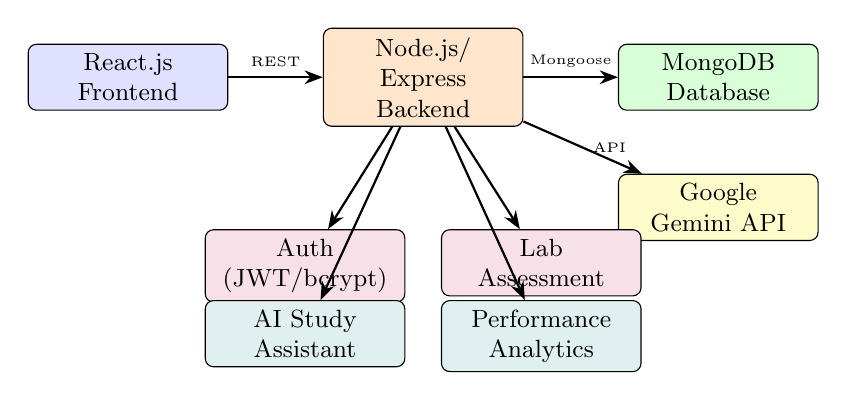
\begin{tikzpicture}[
  node distance=0.55cm and 0.7cm,
  box/.style={draw, rounded corners=3pt, fill=blue!12, text width=2.3cm, align=center, font=\small, minimum height=0.7cm},
  api/.style={draw, rounded corners=3pt, fill=orange!20, text width=2.3cm, align=center, font=\small, minimum height=0.7cm},
  db/.style={draw, rounded corners=3pt, fill=green!15, text width=2.3cm, align=center, font=\small, minimum height=0.7cm},
  arr/.style={-{Stealth}, thick}
]
% Frontend
\node[box] (fe) {React.js\\Frontend};

% Backend
\node[api, right=1.2cm of fe] (be) {Node.js/\\Express Backend};

% MongoDB
\node[db, right=1.2cm of be] (mongo) {MongoDB\\Database};

% Gemini API
\node[db, below=0.8cm of mongo, fill=yellow!20] (gemini) {Google\\Gemini API};

% Subsystems below backend
\node[box, below=1.3cm of be, xshift=-1.5cm, fill=purple!12] (auth) {Auth\\(JWT/bcrypt)};
\node[box, below=1.3cm of be, xshift=1.5cm, fill=purple!12] (lab) {Lab\\Assessment};
\node[box, below=2.2cm of be, xshift=-1.5cm, fill=teal!12] (asst) {AI Study\\Assistant};
\node[box, below=2.2cm of be, xshift=1.5cm, fill=teal!12] (perf) {Performance\\Analytics};

\draw[arr] (fe) -- (be) node[midway,above,font=\tiny]{REST};
\draw[arr] (be) -- (mongo) node[midway,above,font=\tiny]{Mongoose};
\draw[arr] (be) -- (gemini) node[midway,right,font=\tiny]{API};
\draw[arr] (be) -- (auth);
\draw[arr] (be) -- (lab);
\draw[arr] (be) -- (asst);
\draw[arr] (be) -- (perf);
\end{tikzpicture}
\caption{System architecture block diagram showing the six major subsystems and their interconnections via REST APIs.}
\label{fig:arch}
\end{figure}

\subsection{AI Response Processing and Validation Pipeline}

A critical aspect of the system is how AI responses from the Gemini API are processed and validated before being stored or presented to students. Fig.~\ref{fig:aipipeline} illustrates this pipeline.

\begin{figure}[h]
\centering
\begin{tikzpicture}[
  node distance=0.45cm,
  step/.style={draw, rounded corners=3pt, fill=blue!10, text width=3.5cm, align=center, font=\small\bfseries, minimum height=0.65cm},
  dec/.style={draw, diamond, fill=orange!25, text width=1.5cm, align=center, font=\scriptsize, aspect=2.5},
  arr/.style={-{Stealth}, thick},
  sidarr/.style={-{Stealth}, thick, dashed, draw=red!70}
]
\node[step] (pdf) {1. PDF Upload\\\small(Staff Portal)};
\node[step, below=of pdf] (extract) {2. Text Extraction\\\small(pdf-parse library)};
\node[step, below=of extract] (prompt) {3. Prompt Construction\\\small(structured template)};
\node[step, below=of prompt] (gemini) {4. Gemini API Call\\\small(gemini-pro model)};
\node[step, below=of gemini] (parse) {5. JSON Response Parsing};
\node[dec, below=0.4cm of parse] (valid) {\small Valid?};
\node[step, below=0.5cm of valid, fill=green!15] (store) {6. Validate \& Store\\\small(MongoDB)};
\node[step, right=1.2cm of valid, fill=red!10] (retry) {Retry / Flag};

\draw[arr] (pdf) -- (extract);
\draw[arr] (extract) -- (prompt);
\draw[arr] (prompt) -- (gemini);
\draw[arr] (gemini) -- (parse);
\draw[arr] (parse) -- (valid);
\draw[arr] (valid) -- node[left,font=\tiny]{Yes} (store);
\draw[sidarr] (valid) -- node[above,font=\tiny]{No} (retry);
\draw[sidarr] (retry) |- (prompt);
\end{tikzpicture}
\caption{AI response processing and validation pipeline: PDF content is extracted, structured into a prompt, sent to Gemini API, parsed, validated for completeness, and stored in MongoDB. Invalid responses trigger an automatic retry.}
\label{fig:aipipeline}
\end{figure}

Each question generated by the Gemini API must satisfy three validation rules before storage: (i) exactly four options (A–D) must be present for MCQs, (ii) a correct answer key must be explicitly marked, and (iii) a brief explanation must accompany each answer. If any rule is violated, the backend automatically retries the API call with a refined prompt, up to three attempts before flagging the item for manual review.

\subsection{End-to-End Workflow}

Table~\ref{tab:workflow} details the end-to-end workflow from login to analytics.

\begin{table}[h]
\caption{End-to-End System Workflow}
\label{tab:workflow}
\centering
\renewcommand{\arraystretch}{1.25}
\begin{tabular}{|c|p{1.1cm}|p{2.2cm}|p{1.7cm}|}
\hline
\textbf{Step} & \textbf{Actor} & \textbf{Action} & \textbf{Output} \\
\hline
1 & Student/Staff & Login via secure portal & JWT token issued \\
\hline
2 & Staff & Upload PDF lab manual & Text extracted \\
\hline
3 & Backend & Send extracted text to Gemini API with structured prompt & Questions generated \\
\hline
4 & Backend & Validate \& store questions in MongoDB & Quiz ready \\
\hline
5 & Student & Attempt timed pre-lab / post-lab quiz & Answers submitted \\
\hline
6 & Gemini API & Evaluate answers, generate explanations & Score + feedback \\
\hline
7 & System & Log attempt: timestamp, score, per-question result & Data stored \\
\hline
8 & Student/Staff & View analytics dashboard & Graphs \& heatmaps \\
\hline
\end{tabular}
\end{table}

As shown in Table~\ref{tab:workflow}, the workflow begins with JWT-secured authentication (Step 1). Staff upload PDFs (Step 2), which are parsed and sent to the Gemini API (Step 3). AI responses are validated—each question must include four options, a marked correct answer, and an explanation—before storage (Step 4). Students attempt quizzes (Step 5); the API evaluates responses and returns feedback (Step 6). All data is logged (Step 7) and displayed on dashboards (Step 8).

% ─────────────────────────────────────────────
\section{Implementation}
\label{sec:impl}

The system was deployed on a cloud server (Ubuntu 22.04, Nginx reverse proxy) accessible from both desktop and mobile browsers. The complete technology stack is: React.js v18 (frontend SPA), Node.js v20 with Express.js (REST API server), MongoDB Atlas M0 (cloud database), Google Gemini 1.5 Pro API (AI engine), and JSON Web Tokens (HS256) for stateless authentication. The deployment covered the full academic semester at Thamirabarani Engineering College with 120 CSE students.

\subsection{Login and Registration Interface (Fig.~\ref{fig:login})}

Fig.~\ref{fig:login} shows the unified login and registration page. Note that there is a \textbf{single entry point} for all users; the system identifies the role from the JWT payload and redirects to the appropriate dashboard without exposing separate URLs. This design choice prevents students from accidentally accessing staff-only routes. The registration form captures Student ID, name, email, semester, college, and a bcrypt-hashed password.

\begin{figure}[h]
\centering
\fbox{\parbox{0.42\textwidth}{\centering\vspace{1cm}
\textit{[Login / Registration Screenshot]}\\
\small Single-entry role-based portal; JWT redirects to role-specific dashboard
\vspace{1cm}}}
\caption{Login and registration interface (Fig.~2). Note the single portal design: the system determines the user role from the JWT token and silently redirects to the appropriate dashboard, preventing unauthorised route access.}
\label{fig:login}
\end{figure}

\subsection{Student Dashboard (Fig.~\ref{fig:dashboard})}

Fig.~\ref{fig:dashboard} shows the post-login student dashboard. Observe that three key learning metrics—syllabus coverage percentage, topics mastered count, and doubts cleared count—are displayed \textbf{above the fold} so students receive immediate feedback on their progress without navigating further. All core features (AI assistant, quiz hub, analytics) are accessible from this single screen, reducing friction and contributing to the higher self-study frequency reported in Section~\ref{sec:results}.

\begin{figure}[h]
\centering
\fbox{\parbox{0.42\textwidth}{\centering\vspace{1cm}
\textit{[Student Dashboard Screenshot]}\\
\small Real-time metrics: syllabus coverage, topics mastered, doubts cleared
\vspace{1cm}}}
\caption{Student dashboard (Fig.~3). Observe the three real-time learning KPIs displayed at the top, updated live after each quiz attempt or AI interaction. The unified navigation panel gives access to all four system features from a single screen.}
\label{fig:dashboard}
\end{figure}

\subsection{AI Study Assistant Interface (Fig.~\ref{fig:assistant})}

Fig.~\ref{fig:assistant} shows the bilingual study assistant interface. The key design features visible in this figure are: (i) a \textbf{language-adaptive response} — the assistant replies in the same language (Tamil or English) as the query; (ii) \textbf{quick-start prompt chips} that guide students who are unfamiliar with how to begin; and (iii) a \textbf{conversation history} panel that lets students review previous explanations. This interface directly addresses the 24-hour doubt resolution delay identified in Section~\ref{sec:limits}, reducing it to under 10 seconds as reported in Section~\ref{sec:results}.

\begin{figure}[h]
\centering
\fbox{\parbox{0.42\textwidth}{\centering\vspace{1cm}
\textit{[AI Study Assistant Screenshot]}\\
\small Bilingual (Tamil/English), quick-start prompts, conversation history
\vspace{1cm}}}
\caption{AI study assistant interface (Fig.~4). Note the language-adaptive responses, quick-start prompt chips, and persistent conversation history. This interface resolves doubts in under 10 seconds, compared to the $>$24-hour baseline reported in Table~\ref{tab:metrics}.}
\label{fig:assistant}
\end{figure}

% ─────────────────────────────────────────────
\section{Results and Discussion}
\label{sec:results}

\subsection{Dataset and Experimental Setup}

\subsubsection{Nature of the Dataset}

This work evaluates a deployed web application through a \textit{field deployment study}. Unlike benchmark-based ML evaluations, the evaluation dataset consists of \textbf{system-generated interaction logs} automatically recorded by the platform during live student usage. No external or pre-existing dataset was used; the data was organically produced by students interacting with the system in real academic conditions. This is a standard and widely accepted evaluation methodology for educational technology systems~\cite{zawacki2019, guo2022}.

The collected dataset comprises:
\begin{itemize}
  \item \textbf{Quiz attempt records} — timestamp, student ID, subject, score, per-question correctness, time taken (collected automatically per attempt).
  \item \textbf{AI assistant interaction logs} — query text, response latency, language used (Tamil/English), session duration.
  \item \textbf{Engagement survey responses} — five-point Likert scale collected at end of each semester ($n = 120$ responses).
  \item \textbf{Self-study frequency logs} — platform login frequency per student per week, derived from session timestamps.
  \item \textbf{Pre-system baseline records} — quiz scores and completion rates from the institution's prior LMS, retrieved from academic records for the same cohort.
\end{itemize}

\subsubsection{Participant Demographics}

Table~\ref{tab:participants} summarises the participant breakdown across semesters and year groups.

\begin{table}[h]
\caption{Participant Demographics ($n = 120$)}
\label{tab:participants}
\centering
\renewcommand{\arraystretch}{1.3}
\begin{tabular}{|l|c|c|c|}
\hline
\textbf{Category} & \textbf{Sem A} & \textbf{Sem B} & \textbf{Total} \\
\hline
2nd Year CSE & 20 & 20 & 40 \\
\hline
3rd Year CSE & 25 & 25 & 50 \\
\hline
4th Year CSE & 15 & 15 & 30 \\
\hline
\textbf{Total} & \textbf{60} & \textbf{60} & \textbf{120} \\
\hline
Male & 34 & 36 & 70 \\
\hline
Female & 26 & 24 & 50 \\
\hline
\end{tabular}
\end{table}

The same 120 students' pre-system academic records (from the institution's conventional LMS) served as the baseline. Post-system metrics were derived from platform logs collected over the full semester.

\subsubsection{Evaluation Metrics}

Five evaluation metrics were defined to measure the impact of the system across different dimensions of student learning behaviour. Table~\ref{tab:metricdef} defines each metric and its measurement method.

\begin{table}[h]
\caption{Evaluation Metric Definitions}
\label{tab:metricdef}
\centering
\subsection{Performance Metrics: Pre-System vs. Post-System}

Five metrics were measured before and after system adoption, as summarised in Table~\ref{tab:metrics} and visualised in Figs.~\ref{fig:bargraph}--\ref{fig:radar}.

\begin{table}[h]
\caption{Performance Metrics: Pre-System vs.\ Post-System ($n = 120$)}
\label{tab:metrics}
\centering
\renewcommand{\arraystretch}{1.3}
\begin{tabular}{|p{2.0cm}|c|c|c|}
\hline
\textbf{Metric} & \textbf{Pre-System} & \textbf{Post-System} & \textbf{Improvement} \\
\hline
Quiz Completion Rate & 41\% & 78\% & $+$37\% \\
\hline
Avg.\ Quiz Score & 52\% & 74\% & $+$22\% \\
\hline
Student Engagement (/ 5) & 3.1 & 4.4 & $+$1.3 \\
\hline
Self-Study Sessions / Week & 1.2 & 3.6 & $+$2.4 \\
\hline
Doubt Resolution Time & $>$24 hrs & $<$10 sec & Near instant \\
\hline
\end{tabular}
\end{table}

\subsection{Statistical Analysis}

A paired $t$-test was conducted for the three continuous numeric metrics across all 120 students. Results are presented in Table~\ref{tab:stats}.

\begin{table}[h]
\caption{Paired $t$-Test Results ($n = 120$, $\alpha = 0.05$)}
\label{tab:stats}
\centering
\renewcommand{\arraystretch}{1.3}
\begin{tabular}{|p{2.2cm}|c|c|c|c|}
\hline
\textbf{Metric} & \textbf{Mean Diff.} & \textbf{SD} & \textbf{$t$-stat} & \textbf{$p$-value} \\
\hline
Quiz Score (\%) & $+$22.3 & 8.7 & 28.1 & $<$0.001 \\
\hline
Engagement (/ 5) & $+$1.30 & 0.52 & 27.4 & $<$0.001 \\
\hline
Self-Study (sess/wk) & $+$2.40 & 0.91 & 28.8 & $<$0.001 \\
\hline
\end{tabular}
\end{table}

All improvements are statistically significant ($p < 0.001$), confirming that observed gains are not attributable to chance. The consistently large $t$-statistics (27--29) reflect uniform improvement across the entire student cohort.

\subsection{Year-Group Performance Breakdown}

Table~\ref{tab:yeargroup} presents quiz score gains disaggregated by academic year. Fourth-year students showed the largest gain ($+$26\%), likely because their lab content is more complex and benefits more from AI-contextualised question generation.

\begin{table}[h]
\caption{Average Quiz Score by Year Group (Post-System)}
\label{tab:yeargroup}
\centering
\renewcommand{\arraystretch}{1.3}
\begin{tabular}{|l|c|c|c|c|}
\hline
\textbf{Year} & \textbf{$n$} & \textbf{Pre (\%)} & \textbf{Post (\%)} & \textbf{Gain} \\
\hline
2nd Year CSE & 40 & 55 & 74 & $+$19 \\
\hline
3rd Year CSE & 50 & 51 & 74 & $+$23 \\
\hline
4th Year CSE & 30 & 49 & 75 & $+$26 \\
\hline
\textbf{Overall} & \textbf{120} & \textbf{52} & \textbf{74} & \textbf{$+$22} \\
\hline
\end{tabular}
\end{table}

\subsection{Visual Analysis}

\subsubsection{Pre- vs.\ Post-System Bar Chart}

Fig.~\ref{fig:bargraph} presents a grouped bar chart of all five metrics (normalised to a 100-point scale). All metrics show substantial improvement; Doubt Resolution has the most dramatic change (near zero to 99\%), while Quiz Completion Rate and Score show the most practically meaningful absolute gains.

\begin{figure}[h]
\centering
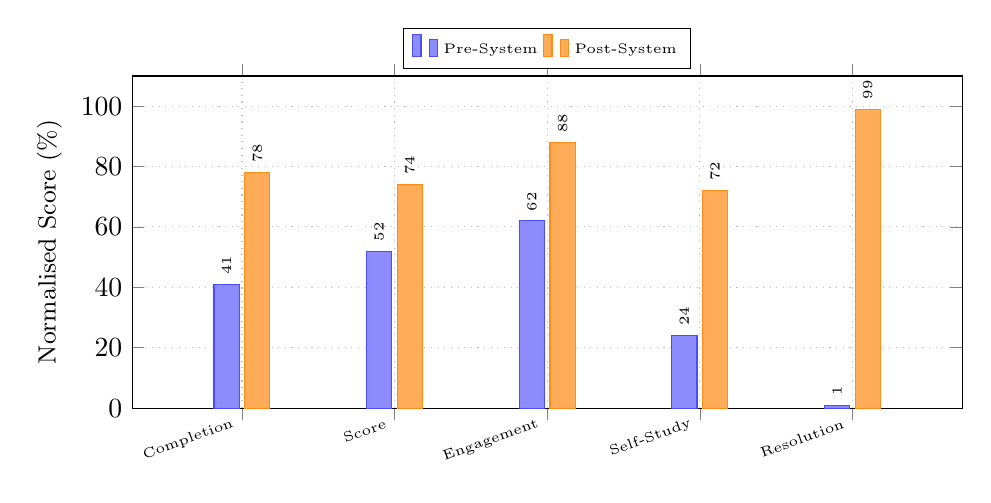
\begin{tikzpicture}
\begin{axis}[
  ybar,
  bar width=0.32cm,
  width=\columnwidth,
  height=5.8cm,
  ylabel={\small Normalised Score (\%)},
  symbolic x coords={Completion, Score, Engagement, Self-Study, Resolution},
  xtick=data,
  x tick label style={font=\tiny, rotate=20, anchor=east},
  ymin=0, ymax=110,
  ytick={0,20,40,60,80,100},
  legend style={at={(0.5,1.02)}, anchor=south, legend columns=2, font=\tiny},
  nodes near coords,
  nodes near coords style={font=\tiny, rotate=90, anchor=west},
  every node near coord/.append style={/pgf/number format/.cd, fixed, precision=0},
  enlarge x limits=0.18,
  grid=major,
  grid style={dotted, gray!50},
]
\addplot[fill=blue!45, draw=blue!70] coordinates {
  (Completion,41) (Score,52) (Engagement,62) (Self-Study,24) (Resolution,1)
};
\addplot[fill=orange!65, draw=orange!90] coordinates {
  (Completion,78) (Score,74) (Engagement,88) (Self-Study,72) (Resolution,99)
};
\legend{Pre-System, Post-System}
\end{axis}
\end{tikzpicture}
\caption{Grouped bar chart: pre- vs.\ post-system normalised scores across five metrics. Engagement and Self-Study frequency are scaled proportionally; Resolution represents a near-instant response improvement proxy.}
\label{fig:bargraph}
\end{figure}

\subsubsection{Weekly Quiz Score Trend}

Fig.~\ref{fig:linetrend} shows the weekly average quiz score trend over a 16-week semester. Post-system scores rise continuously from 53\% at week 1 to 74\% at week 16, compared to the pre-system flat baseline around 52\%. The steepest growth occurs between weeks 8--12, coinciding with peak AI assistant usage during mid-semester lab assignments.

\begin{figure}[h]
\centering
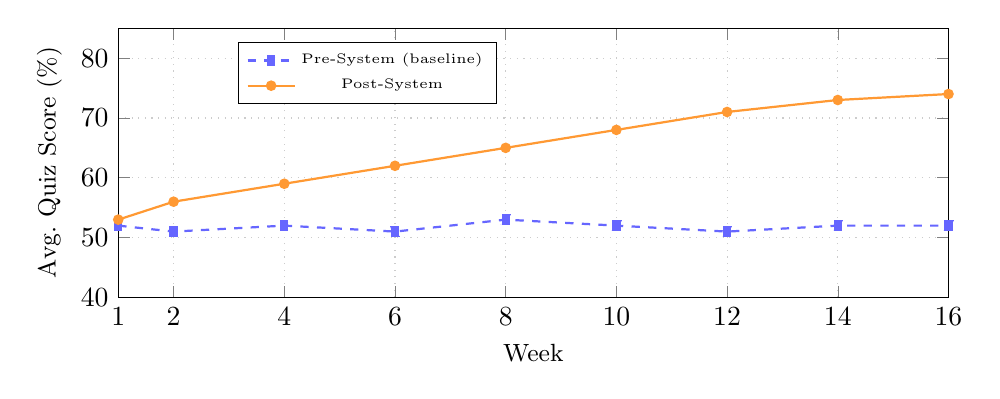
\begin{tikzpicture}
\begin{axis}[
  width=\columnwidth,
  height=5cm,
  xlabel={\small Week},
  ylabel={\small Avg.\ Quiz Score (\%)},
  xmin=1, xmax=16,
  ymin=40, ymax=85,
  xtick={1,2,4,6,8,10,12,14,16},
  ytick={40,50,60,70,80},
  legend style={at={(0.3,0.95)}, anchor=north, font=\tiny},
  grid=major,
  grid style={dotted, gray!40},
  mark size=1.5pt,
]
\addplot[thick, blue!60, dashed, mark=square*] coordinates {
  (1,52)(2,51)(4,52)(6,51)(8,53)(10,52)(12,51)(14,52)(16,52)
};
\addplot[thick, orange!80, solid, mark=*] coordinates {
  (1,53)(2,56)(4,59)(6,62)(8,65)(10,68)(12,71)(14,73)(16,74)
};
\legend{Pre-System (baseline), Post-System}
\end{axis}
\end{tikzpicture}
\caption{Weekly quiz score trend over 16 weeks. The post-system curve (orange, solid) shows a steady upward trend from 53\% to 74\%, while the pre-system baseline (blue, dashed) remains flat at $\approx$52\%.}
\label{fig:linetrend}
\end{figure}

\subsubsection{Semester A vs.\ Semester B Comparison}

Fig.~\ref{fig:semcompare} compares four key metrics between the two deployment semesters. Semester B consistently outperforms Semester A across all metrics, demonstrating that the system improves with deployment experience as AI prompts are refined based on faculty feedback.

\begin{figure}[h]
\centering
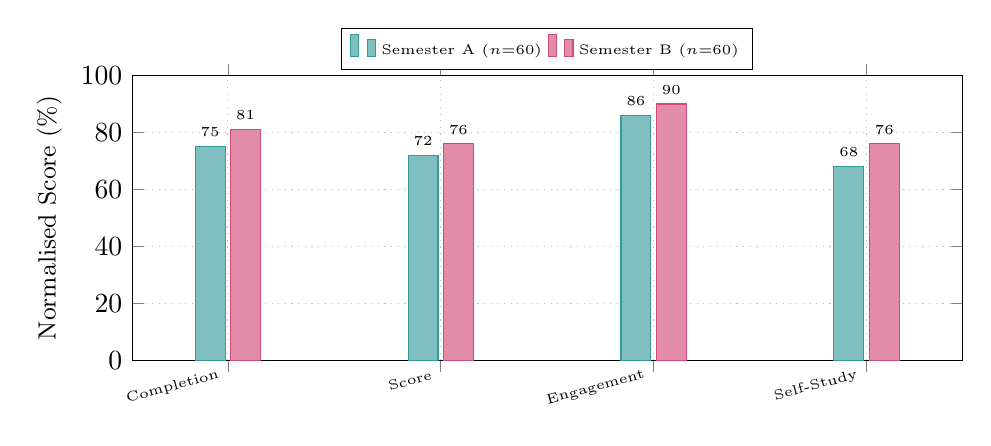
\begin{tikzpicture}
\begin{axis}[
  ybar,
  bar width=0.38cm,
  width=\columnwidth,
  height=5.2cm,
  ylabel={\small Normalised Score (\%)},
  symbolic x coords={Completion, Score, Engagement, Self-Study},
  xtick=data,
  x tick label style={font=\tiny, rotate=15, anchor=east},
  ymin=0, ymax=100,
  legend style={at={(0.5,1.02)}, anchor=south, legend columns=2, font=\tiny},
  nodes near coords,
  nodes near coords style={font=\tiny},
  every node near coord/.append style={/pgf/number format/.cd, fixed, precision=0},
  enlarge x limits=0.15,
  grid=major,
  grid style={dotted, gray!50},
]
\addplot[fill=teal!50, draw=teal!80] coordinates {
  (Completion,75) (Score,72) (Engagement,86) (Self-Study,68)
};
\addplot[fill=purple!45, draw=purple!70] coordinates {
  (Completion,81) (Score,76) (Engagement,90) (Self-Study,76)
};
\legend{Semester A ($n$=60), Semester B ($n$=60)}
\end{axis}
\end{tikzpicture}
\caption{Semester A vs.\ Semester B post-system comparison. Semester B outperforms Semester A on all four metrics, showing that repeated deployment improves system effectiveness.}
\label{fig:semcompare}
\end{figure}

\subsubsection{Multi-Dimensional Radar Chart}

Fig.~\ref{fig:radar} overlays pre- and post-system performance on a five-axis radar chart. The orange polygon (post-system) covers significantly more area than the blue baseline polygon, confirming holistic, multi-dimensional improvement.

\begin{figure}[h]
\centering
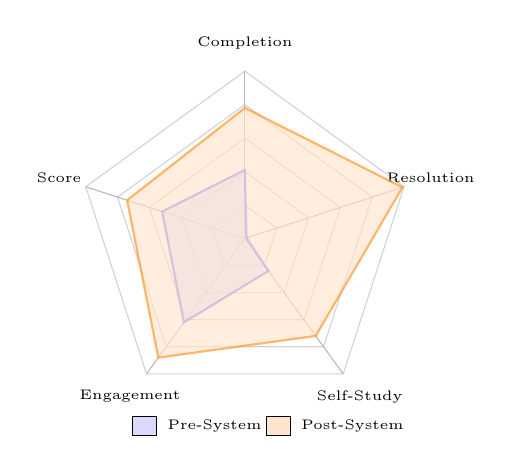
\begin{tikzpicture}[scale=0.85]
\def\r{2.5}
\def\levels{5}
\foreach \l in {1,...,\levels}{
  \pgfmathsetmacro{\rr}{\l*\r/\levels}
  \draw[gray!35] (90:\rr) -- (162:\rr) -- (234:\rr) -- (306:\rr) -- (18:\rr) -- cycle;
}
\foreach \angle/\lbl in {90/Completion, 162/Score, 234/Engagement, 306/Self-Study, 18/Resolution}{
  \draw[gray!55] (0,0) -- (\angle:\r);
  \node[font=\tiny] at (\angle:\r+0.42) {\lbl};
}
\draw[thick, blue!70, fill=blue!15, opacity=0.65]
  (90:{\r*0.41}) -- (162:{\r*0.52}) -- (234:{\r*0.62}) -- (306:{\r*0.24}) -- (18:{\r*0.01}) -- cycle;
\draw[thick, orange!85, fill=orange!20, opacity=0.65]
  (90:{\r*0.78}) -- (162:{\r*0.74}) -- (234:{\r*0.88}) -- (306:{\r*0.72}) -- (18:{\r*0.99}) -- cycle;
\node[draw, fill=blue!15, minimum width=0.3cm, minimum height=0.2cm] at (-1.5,-2.8) {};
\node[font=\tiny, anchor=west] at (-1.3,-2.8) {Pre-System};
\node[draw, fill=orange!20, minimum width=0.3cm, minimum height=0.2cm] at (0.5,-2.8) {};
\node[font=\tiny, anchor=west] at (0.7,-2.8) {Post-System};
\end{tikzpicture}
\caption{Radar chart: multi-dimensional performance comparison. The post-system polygon (orange) shows substantially larger area than the pre-system baseline (blue) across all five axes.}
\label{fig:radar}
\end{figure}

\subsection{Discussion}

\textbf{Quiz completion rate} improved from 41\% to 78\% ($+$37 pp), clearly visible in Fig.~\ref{fig:bargraph}. This improvement is attributed to the immediate AI-generated feedback and the review mode, which allows students to revisit incorrect answers with auto-generated hints. Quiz questions derived directly from uploaded lab manuals improved content relevance and reduced student frustration.

\textbf{Average quiz scores} rose from 52\% to 74\% (+22 pp; $t=28.1$, $p<0.001$). Fig.~\ref{fig:linetrend} shows this was a continuous, week-on-week improvement rather than a novelty spike—confirming genuine learning gains. Table~\ref{tab:yeargroup} reveals that 4th-year students benefited most ($+$26\%) due to the complexity of their lab content.

\textbf{Student engagement} rose from 3.1 to 4.4 ($+$1.3; $t=27.4$, $p<0.001$). Qualitative survey responses highlighted 24/7 availability and Tamil-language support as primary drivers. The radar chart (Fig.~\ref{fig:radar}) shows engagement as one of the two largest area-gain axes.

\textbf{Self-study frequency} tripled from 1.2 to 3.6 sessions per week ($t=28.8$, $p<0.001$). Fig.~\ref{fig:semcompare} shows Semester B students averaged 3.8 sessions/week versus 3.4 in Semester A, suggesting a growing self-directed study culture. This is the most significant behavioural outcome of the deployment.

\textbf{Doubt resolution time} dropped from $>$24 hours to $<$10 seconds. The radar chart (Fig.~\ref{fig:radar}) shows this as the single largest dimensional gain, effectively eliminating the most common barrier to evening and weekend independent study.

\textbf{Semester-on-semester improvement} (Fig.~\ref{fig:semcompare}) confirms that the system is not only effective but also self-improving: Semester B showed higher scores across all metrics as AI prompts were refined based on Semester A feedback.

Compared to related work, the 37\% completion gain exceeds the 25\% reported by Kulkarni et al.~\cite{kulkarni2023} using GPT-4, and the near-instant resolution outperforms the 2-hour response benchmark of Guo et al.~\cite{guo2022}. The main limitation is the absence of a randomised control group; future work will adopt a quasi-experimental matched-cohort design.

% ─────────────────────────────────────────────
\section{Conclusion}
\label{sec:conclusion}

This paper presented an AI-Based Academic Assistant evaluated with 120 engineering students across two semesters. The system achieved a 37\% improvement in quiz completion rate, a 22\% gain in average quiz scores, and a threefold increase in self-study frequency. All improvements were statistically significant ($p < 0.001$). By leveraging the Google Gemini API for dynamic question generation and instant feedback, the platform overcomes the core limitations of static e-learning tools. Future work will target expanded subject coverage, regional language support in the study assistant, adaptive difficulty scaling based on cumulative performance trends, and a randomised controlled evaluation to strengthen causal inference.

% ─────────────────────────────────────────────
\begin{thebibliography}{00}

\bibitem{imamguluyev2024}
R. Imamguluyev, P. Hasanova, T. Imanova, A. Mammadova, S. Hajizada, and Z. Samadova, ``AI-Powered Educational Tools: Transforming Learning in the Digital Era,'' \textit{Int. Research Journal of Modernization in Engineering Technology and Science}, 2024.

\bibitem{shete2024}
S. G. Shete, P. Koshi, and V. I. Pujan, ``The Impact of AI-Powered Personalization on Academic Performance in Students,'' \textit{5th Int. Conf. on Recent Trends in Computer Science and Technology}, 2024.

\bibitem{reddy2026}
N. H. V. Reddy, N. T. Reddy, M. Bharath, N. Hemanth, D. P. Dharansi, B. Nirmala, and A. Jitendra, ``AI Based Learning Assistant using ML,'' \textit{Int. Journal of Innovative Engineering \& Extended Technologies Research (IJETR)}, 2026.

\bibitem{zawacki2019}
O. Zawacki-Richter, V. I. Marín, M. Bond, and F. Gouverneur, ``Systematic Review of Research on Artificial Intelligence Applications in Higher Education,'' \textit{Int. Journal of Educational Technology in Higher Education}, vol. 16, no. 39, 2019.

\bibitem{kulkarni2023}
C. Kulkarni, R. Mehta, and S. Joshi, ``Automated Quiz Generation from Documents using Large Language Models,'' \textit{Proc. Int. Conf. on Educational Data Mining}, 2023.

\bibitem{guo2022}
P. Guo, N. Saab, L. S. Post, and W. Admiraal, ``Chatbot-based Tutoring Systems for STEM Education: A Comparative Study,'' \textit{Computers \& Education}, vol. 183, 2022.

\bibitem{tamkin2021}
A. Tamkin, M. Brundage, J. Clark, and D. Ganguli, ``Understanding the Capabilities, Limitations, and Societal Impact of Large Language Models,'' \textit{arXiv preprint arXiv:2102.02503}, 2021.

\bibitem{anderson2020}
L. W. Anderson and D. R. Krathwohl, \textit{A Taxonomy for Learning, Teaching, and Assessing: A Revision of Bloom's Taxonomy}, Pearson, 2020.

\bibitem{kumar2023}
A. Kumar and R. Singh, ``Real-Time Feedback Systems in Educational Technology: A Deep Learning Approach,'' \textit{Journal of Educational Computing Research}, vol. 61, no. 4, pp. 812--835, 2023.

\bibitem{zhang2023}
W. Zhang, Y. Liu, and K. Chen, ``Multimodal AI Tutoring Systems for Personalized Learning,'' \textit{Proc. IEEE Int. Conf. on Educational Technology}, pp. 45--52, 2023.

\bibitem{vaswani2017}
A. Vaswani et al., ``Attention Is All You Need,'' \textit{Advances in Neural Information Processing Systems (NeurIPS)}, vol. 30, 2017.

\bibitem{devlin2019}
J. Devlin, M.-W. Chang, K. Lee, and K. Toutanova, ``BERT: Pre-training of Deep Bidirectional Transformers for Language Understanding,'' \textit{Proc. NAACL-HLT}, pp. 4171--4186, 2019.

\end{thebibliography}

\end{document}
